% Dokumenteinstellungen und Anpassungen
\documentclass[chapterprefix=false, 12pt, a4paper, oneside, parskip=half, listof=totoc, bibliography=totoc, numbers=noendperiod]{article}

%\renewcommand{\familydefault}{\sfdefault}
%\usepackage{helvet}


%Anpassung der Seitenränder (Standard bottom ca. 52mm abzüglich von ca. 4mm für die nach oben rechts gewanderte Seitenzahl)
\usepackage[bottom=20mm,left=25mm,right=25mm, top=25mm]{geometry}

\usepackage{csquotes}
\usepackage[round,sort&compress, authoryear]{natbib}
\bibliographystyle{plainnat}

%Tweaks für scrbook
\usepackage{scrhack}

\usepackage{tabularx} % in the preamble

%Blindtext
\usepackage{blindtext}

%Erlaubt unter anderem Umbrüche captions
\usepackage{caption}

%Stichwortverzeichnis
\usepackage{imakeidx}

%Kompakte Listen
\usepackage{paralist}

%Zitate besser formatieren und darstellen
\usepackage{epigraph}

%Glossar, Stichwortverzeichnis (Akronyme werden als eigene Liste aufgeführt)
\usepackage[toc, acronym]{glossaries}

%Anpassung von Kopf- und Fußzeile
%beeinflusst die erste Seite des Kapitels
\usepackage[automark,headsepline]{scrlayer-scrpage}
%\input{resources/styles/header_footer}
\setlength{\parindent}{0em}

%\renewcommand\chapter{\thispagestyle{plain}}

%Auskommentieren für die Verkleinerung des vertikalen Abstandes eines neuen Kapitels
%\renewcommand*{\chapterheadstartvskip}{\vspace*{.25\baselineskip}}
%\renewcommand*{\chapterheadendvskip}{\vspace*{.25\baselineskip}}

%Zeilenabstand 1,5
\usepackage[onehalfspacing]{setspace}

%Verbesserte Darstellung der Buchstaben zueinander
\usepackage[stretch=10]{microtype}

%Deutsche Bezeichnungen für angezeigte Namen (z.B. Inhaltsverzeichnis etc.)
\usepackage[ngerman]{babel}

%Unterstützung von Umlauten und anderen Sonderzeichen (UTF-8)
\usepackage{lmodern}
\usepackage[utf8]{luainputenc}
\usepackage[T1]{fontenc}
\usepackage[ngerman]{babel}
\setlength{\emergencystretch}{1em}

%Einfachere Zitate
\usepackage{epigraph}

%Unterstützung der H Positionierung (keine automatische Verschiebung eingefügter Elemente)
\usepackage{float}

%Erlaubt Umbrüche innerhalb von Tabellen
\usepackage{tabularx}

%Erlaubt Seitenumbrüche innerhalb von Tabellen
\usepackage{longtable}

%Erlaubt die Darstellung von Sourcecode mit Highlighting
\usepackage{listings}

%Definition eigener Farben bei Nutzung eines selbst vergebene Namens
\usepackage[table,xcdraw]{xcolor}

%Vektorgrafiken
\usepackage{tikz}

%Grafiken (wie jpg, png, etc.)
\usepackage{graphicx}

%Grafiken von Text umlaufen lassen
\usepackage{wrapfig}

%Ermöglicht Verknüpfungen innerhalb des Dokumentes (e.g. for PDF), Links werden durch "hidelink" nicht explizit hervorgehoben
\usepackage[hidelinks,german]{hyperref}

\setlength{\headheight}{18pt}

%Zusätzliche Farben
\definecolor{darkgreen}{RGB}{0,100,0}
\setlength{\emergencystretch}{15pt}

%Umbenennungen
\renewcommand{\lstlistlistingname}{Quelltextverzeichnis}

\renewcommand{\lstlistingname}{Codeauszug}
\lstset{
	language=Java,
	numbers=left,
	columns=fullflexible,
	aboveskip=5pt,
	belowskip=10pt,
	basicstyle=\small\ttfamily,
	backgroundcolor=\color{black!5},
	commentstyle=\color{darkgreen},
	keywordstyle=\color{blue},
	stringstyle=\color{gray},
	showspaces=false,
	showstringspaces=false,
	showtabs=false,
	xleftmargin=16pt,
	xrightmargin=0pt,
	framesep=5pt,
	framerule=3pt,
	frame=leftline,
	rulecolor=\color{green},
	tabsize=2,
	breaklines=true,
	breakatwhitespace=true,
	prebreak={\mbox{$\hookleftarrow$}}
}

%Anpassungen für das Abkürzungsverzeichnis
\newglossarystyle{dottedlocations}{%
	\renewcommand*{\glossaryentryfield}[5]{%
		\item[\glsentryitem{##1}\glstarget{##1}{##2}] \emph{##3}%
		\unskip\leaders\hbox to 2.9mm{\hss.}\hfill##5}%
	\renewcommand*{\glsgroupskip}{}%
}


\usepackage{graphicx}
\usepackage{subcaption}
\usepackage{float}
\usepackage{color}
\usepackage{listings}
\usepackage{eso-pic}
\usepackage{caption}
\usepackage{csquotes}
\usepackage{pgfplots}

\definecolor{myblue}{HTML}{92dcec}

\newcommand\BackgroundPic{%
\put(0,0){%
\parbox[b][\paperheight]{\paperwidth}{%
\vfill
\centering

\includegraphics[width=\paperwidth,height=\paperheight,%
keepaspectratio]{resources/images/deckblatt.jpg}%
\vfill
}}}


\makeatletter
\newcommand*{\germanTitle}[1]{\gdef\@germanTitle{#1}}
\newcommand*{\englishTitle}[1]{\gdef\@englishTitle{#1}}
\newcommand*{\gradeType}[1]{\gdef\@gradeType{#1}}
\newcommand*{\firstExaminer}[1]{\gdef\@firstExaminer{#1}}
\newcommand*{\secondExaminer}[1]{\gdef\@secondExaminer{#1}}
\newcommand*{\matrikelnr}[1]{\gdef\@matrikelnr{#1}}
\newcommand*{\authorBirthplace}[1]{\gdef\@authorBirthplace{#1}}
\newcommand*{\submitDate}[1]{\gdef\@submitDate{#1}}
\newcommand*{\discipline}[1]{\gdef\@discipline{#1}}
\newcommand*{\courseOfStudies}[1]{\gdef\@courseOfStudies{#1}}
\newcommand*{\authorLastname}[1]{\gdef\@authorLastname{#1}}
\newcommand*{\authorFirstname}[1]{\gdef\@authorFirstname{#1}}


\renewcommand*{\maketitle}{
	\begin{titlepage}
		\newgeometry{left=3.8cm,right=2.5cm,top=4.6cm,bottom=2.5cm}
			\begingroup
				\fontsize{44pt}{46pt}\selectfont
				{\bfseries Seminarfacharbeit}
			\endgroup

			\vskip 1.44cm

			\begingroup
			\fontsize{8pt}{6pt}\selectfont
			Titel der Arbeit // Title of Thesis
			\endgroup

			\vskip -0.02cm

			\begingroup
			\fontsize{16pt}{16pt}\selectfont
			{\bfseries \@germanTitle\par}
			{\bfseries \@englishTitle\par}
			\endgroup
			\vskip -0.1cm

			\noindent\rule{15cm}{0.4pt}
			
			\vskip 0.05cm

			\begingroup
			\fontsize{8pt}{6pt}\selectfont
			Akademischer Abschlussgrad: Grad, Fachrichtung (Abkürzung) // Degree
			\endgroup

			\vskip -0.15cm

			\begingroup
			\fontsize{12pt}{14pt}\selectfont
				{\@gradeType}
			\endgroup
			\vskip -0.15cm

			\noindent\rule{15cm}{0.4pt}
			
			\vskip 0.05cm

			\begingroup
			\fontsize{8pt}{6pt}\selectfont
			Autorenname, Geburtsort // Name, Place of Birth
			\endgroup

			\vskip -0.15cm

			\begingroup
			\fontsize{12pt}{14pt}\selectfont
				{\@authorFirstname} {\@authorLastname}, {\@authorBirthplace}
			\endgroup
			\vskip -0.15cm

			\noindent\rule{15cm}{0.4pt}
			
			\vskip 0.05cm

			\begingroup
			\fontsize{8pt}{6pt}\selectfont
			Studiengang // Course of Study
			\endgroup

			\vskip -0.15cm

			\begingroup
			\fontsize{12pt}{14pt}\selectfont
				{\@courseOfStudies}
			\endgroup
			\vskip -0.15cm

			\noindent\rule{15cm}{0.4pt}
			
			\vskip 0.05cm

			\begingroup
			\fontsize{8pt}{6pt}\selectfont
			Fachbereich // Department
			\endgroup

			\vskip -0.15cm

			\begingroup
			\fontsize{12pt}{14pt}\selectfont
				{\@discipline}
			\endgroup
			\vskip -0.15cm

			\noindent\rule{15cm}{0.4pt}
			
			\vskip 0.05cm

			\begingroup
			\fontsize{8pt}{6pt}\selectfont
			Erstprüferin/Erstprüfer // First Examiner
			\endgroup

			\vskip -0.15cm

			\begingroup
			\fontsize{12pt}{14pt}\selectfont
				{\@firstExaminer}
			\endgroup
			\vskip -0.15cm

			\noindent\rule{15cm}{0.4pt}
			
			\vskip 0.05cm

			\begingroup
			\fontsize{8pt}{6pt}\selectfont
			Zweitprüferin/Zweitprüfer // Second Examiner
			\endgroup

			\vskip -0.15cm

			\begingroup
			\fontsize{12pt}{14pt}\selectfont
				{\@secondExaminer}
			\endgroup
			\vskip -0.15cm

			\noindent\rule{15cm}{0.4pt}
			
			\vskip 0.05cm

			\begingroup
			\fontsize{8pt}{6pt}\selectfont
			Abgabedatum // Date of Submission
			\endgroup

			\vskip -0.15cm

			\begingroup
			\fontsize{12pt}{14pt}\selectfont
				{\@submitDate}
			\endgroup
			\vskip -0.15cm

			\noindent\rule{15cm}{0.4pt}
		\restoregeometry
	\end{titlepage}
}
\makeatother

% Variablen für das Deckblatt
\gradeType{Abitur 2021}
\germanTitle{Face Recognition mit Hilfe von Künstlicher Intelligenz}
\englishTitle{}
\authorFirstname{Kevin}
\authorLastname{Pagenkämper}
\authorBirthplace{Nordhorn}
\discipline{Technik und Ethik}
\courseOfStudies{Informatik}
\matrikelnr{112}
\submitDate{02.03.2020}
\firstExaminer{Andre Nixdorf}
\secondExaminer{Henrike Schnöing}


\makeatletter

\newcommand*{\place}[1]{\gdef\@place{#1}}

\newcommand*{\makeeidesstatt}{
	\begin{titlepage}
		\newgeometry{left=3.8cm,right=2.5cm,top=8cm,bottom=2.5cm}
			\begingroup
			\fontsize{18pt}{20pt}\selectfont
			{\bfseries Eidesstattliche Versicherung}
			\endgroup

			\vskip 0.8cm

			\begingroup
			\fontsize{12pt}{14pt}\selectfont
				{\@authorLastname} {\@authorFirstname}
			\endgroup

			\vskip -0.5cm

			\noindent\rule{15cm}{0.4pt}

			\vskip -0.4cm

			\begingroup
			\fontsize{8pt}{6pt}\selectfont
			Name, Vorname // Name, First Name
			\endgroup

			\vskip 0.6cm
			\begingroup
			\fontsize{10.5pt}{11.5pt}\selectfont
			Ich versichere hiermit an Eides statt, dass ich die vorliegende Seminarfacharbeit mit dem Titel
			\endgroup

			\begingroup
			\fontsize{16pt}{18pt}\selectfont
			{\bfseries \@germanTitle}
			\endgroup

			\begingroup
			\fontsize{10.5pt}{11.5pt}\selectfont
			selbstständig und ohne unzulässige fremde Hilfe erbracht habe. Ich habe keine anderen als die angegebenen Quellen und Hilfsmittel benutzt sowie wörtliche und sinngemäße Zitate kenntlich gemacht. Die Arbeit hat in gleicher oder ähnlicher Form noch keiner Prüfungsbehörde vorgelegen.
			\endgroup

			\vskip 0.8cm

			{
			\fontsize{12pt}{14pt}\selectfont
			{\@place}, den {\today}
			}

			\vskip -0.5cm

			\noindent\rule{15cm}{0.4pt}

			\vskip -0.3cm

			\begingroup
			\fontsize{8pt}{6pt}\selectfont
			Ort, Datum, Unterschrift // Place, Date, Signature
			\endgroup


		\restoregeometry
	\end{titlepage}
}
\makeatother

\place{Nordhorn}


\lstset{literate=%
  {Ö}{{\"O}}1
  {Ä}{{\"A}}1
  {Ü}{{\"U}}1
  {ß}{{\ss}}1
  {ü}{{\"u}}1
  {ä}{{\"a}}1
  {ö}{{\"o}}1
}

% Javascript als Sprache für die lstings
\lstdefinelanguage{JavaScript}{
  keywords={typeof, new, true, false, catch, function, return, null, catch, switch, var, if, in, while, do, else, case, break, that, globals, let, const},
  keywordstyle=\color{blue}\bfseries,
  ndkeywords={class, export, boolean, throw, implements, import, this},
  ndkeywordstyle=\color{darkgray}\bfseries,
  identifierstyle=\color{black},
  sensitive=false,
  comment=[l]{//},
  morecomment=[s]{/*}{*/},
  commentstyle=\color{gray}\ttfamily,
  stringstyle=\color{red}\ttfamily,
  morestring=[b]',
  morestring=[b]"
}
\lstset{
    language=JavaScript,
    numbers=none,
    frame=leftline,
    tabsize=2,
    rulesepcolor=\color{gray},
    rulecolor=\color{black},
    captionpos=b,
    breaklines=true,
    breakatwhitespace=false,
}

% Neuer Befehl um Subsubsubkapitel schreiben zu können
\newcommand{\subsubsubsection}[1]{\paragraph{#1}\mbox{}\\}
\setcounter{secnumdepth}{4}
\setcounter{tocdepth}{4}
\usepackage{fontspec}
\setmainfont{Arial}

\begin{document}

% Entfernen der Seitenzahlen und BackroundPic als Hintergrund nutzen
\pagenumbering{gobble}
\AddToShipoutPicture{\BackgroundPic}

% Titelblatt erzeugen
\maketitle
\newpage

% Eidesstattliche Erklärung erzeugen
\makeeidesstatt
\thispagestyle{empty}

% Abstract und Inhaltsverzeichnisse einfügen (Numerierung römisch ab Inhaltsverzeichnis)
%\section*{Abstract}
\label{sec:abstract}

\ClearShipoutPicture
\thispagestyle{empty}
\newpage
\pagenumbering{Roman}
\tableofcontents
%\newpage
%\listoffigures
\newpage

% Kapitel einfügen
\pagenumbering{arabic}
% „ = Alt + 0132
% “ = Alt + 0147
\section{Einleitung}
\label{sec:einleitung}
Vor ungefähr 64 Jahren wurde das erste Programm, welches speziell zur Problemlösung und nachahmung eines Menschen entwickelt wurde, von Herbert Alexander Simon und Allen Newell geschrieben. Dieses Programm war Quellen zufolge das erste Programm welches der Definition von Künstlicher Intelligenz, ein Programm welches speziell dafür entwickelt wurde die Fähigkeiten eines Menschen Nachzuahmen, gerecht wurde [vgl. \ref{bib:LogicTheorist}] wobei zu dem Zeitpunkt der Entwicklung dieser das Wort "Künstliche Intelligenz" [folgend auch als KI bezeichnet] noch nicht existierte bzw. nicht in diesem Kontext verwendet wurde [vgl. \ref{LogicTheorist:Wikipedia}]. Seitdem hat sich das Thema KI sowohl in der Hardware aber auch in der Software stark weiterentwickelt. Wo Künstliche Intelligenzen früher nur mit einfachen Zahlen arbeiten konnten, können einige mittlerweile Personen, Gesichter, Objekte und andere Dinge identifizieren und differenzieren. Doch auch hierbei gibt es Probleme die seit der Entwicklung von Gesichtserkennungsprogrammen in den 1960er nicht vollständig gelöst werden konnten, weshalb es bisher auch keine KI gibt welche keine Mängel aufweist. Und gibt es eine KI die momentan eine erfolgschance von 100\% hat ist dies aus dem Grund so, dass sie ihrem Schwachpunkt noch nicht begegnet ist. In dieser Facharbeit wird das Thema der Gesichtserkennung, zu engl. "Face recognition", behandelt. Bei dieser Art der Anwendung von Künstlicher Intelligenz liegt die Schwierigkeit besonders bei Unschärfe, Fragmenten, Verzerrungen und Ähnlichkeiten von Objekten und besonders von Gesichtern. Dies ist z.B. bei Zwillingen der Fall an dem viele Systeme noch heute scheitern. Zudem wird die Theorie von Face Recognition mit Hilfe von Künstlicher Intelligenz erklärt, mit praktischen Beispielen erläutert und auf ethischer Basis analysiert.
\newpage
% Theorie Einführung
\section{Theoretischer Hintergrund}
\label{sec:theorie}
    \subsection{Definition Künstliche Intelligenz}
    \label{subsec:definiton_kuenstliche_intelligenz}
    Das Interesse an dem Thema Künstliche Intelligenz sowie die Einsatzmöglichkeiten steigen stetig an. Künstliche Intelligenz ist ein sehr großes Thema. Für eine grobe Wiedergabe worum es in diesem Thema geht liefert Wikipedia einen guten Einstieg: 
    \textit{\enquote{Künstliche Intelligenz [...] ist ein Teilgebiet der Informatik, welches sich mit der Automatisierung intelligenten Verhaltens und dem maschinellen Lernen befasst.}} [siehe \ref{wiki:KuenstlicheIntelligenz}]\\

    Mit dieser Aussage kann man Künstliche Intelligenz im groben Beschreiben. Etwas genauer beschreibt es Klaus Mainzer in seinem Buch \enquote{Künstliche Intelligenz - Wann übernehme die Maschinen?} [siehe \ref{book:KI_WannUebernehmenDieMaschinen}]. In diesem geht er auf die Definition der Intelligenz von Systemen ein. Laut ihm heißt ein System intelligent \textit{\enquote{wenn es selbstständig und effizient Probleme lösen kann. Der Grad der Intelligenz hängt vom Grad der Selbstständigkeit, dem Grad der Komplexität des Problems und dem Grad der Effizienz des Problemlösungsverfahrens ab}} [siehe S.3 in \ref{book:KI_WannUebernehmenDieMaschinen}].\\
    
    Um es einmal auf den Punkt zu bringen, bezeichnet \enquote{Künstliche Intelligenz} ein System welches selbstständig lernen und effizient Probleme lösen kann und zudem noch lernfähig ist.

    \subsection{Wie funktioniert eine Künstliche Intelligenz?}
    \label{subsec:wie_funktioniert_eine_kuenstliche_intelligenz}
    Künstliche Intelligenzen funktionieren je nach Abwandlung etwas verschieden aber ähneln sich dennoch in ihrem Aufbau. In dieser Arbeit werden die sogenannten Neuronalen Netzwerke, welche in den meisten Systemen Anwendung finden, behandelt. Dennoch werden zunächst die beiden Definitionen \enquote{Deep Learning} und \enquote{Machine Learning} behandelt, da diese eine große Rolle im Bereich KI spielen.

        \subsubsection{Deep Learning}
        \label{subsubsec:deep_learning}
            Deep Learning ist ein Lernverfahren für eine KI welches selbst auch als Machine Learning bezeichnet werden kann. In einem solchen Verfahren lernt die Software mit Hilfe eines programmierten Neuronalen Netzwerk um im Nachhinein präzise Ausgaben zu tätigen [vgl. \ref{subsec:machine_learning_and_deep_learning}]. Diese spezielle Art des Lernens wird für die Neuronalen Netze verwendet die in dieser Arbeit hauptsächlich behandelt werden. In einem späteren Abschnitt wird das Trainieren eines Neuronalen Netzes noch einmal genauer erklärt. [siehe \ref{subsubsec:trainieren_eines_neuronalen_netzes}]

        \subsubsection{Machine Learning}
        \label{subsubsec:machnine_learning}
            \enquote{Algorithms that parse data, learn from that data, and then apply what they’ve learned to make informed decisions} [siehe \ref{subsec:machine_learning_and_deep_learning}]. Sinngemäß übersetzt heißt dieser Satz \enquote{Algorythmen die Daten analysieren, von diesen lernen, und ihr erlerntes Wissen zu nutzen um sachkundige Entscheidungen zu treffen}. Dies ist die Grunddefinition zu Machine Learning, zu deutsch Maschinelles Lernen, auf die sich in dieser Arbeit berufen wird.\\
            Um dies an einem realen Beispiel zu veranschaulichen kann man sich Streaming Dienste wie Spotify, Deezer, Netflix oder Amazon Prime nahmen. Hierbei sei gesagt, dass die folgende Theorie zur Verarbeitung von Daten nicht unbedingt der Wirklichkeit entsprechen muss. Dies ist nur ein Ansatz auf welche Art und Weise ein Machine Learning Ansatz umsetzbar ist.\\

            Für das Maschinelle Lernen ist keine komplexe Struktur nötig. Wenn man einfach nur ein System möchte welches einem Nutzer z.B. auf der Seite Netflix neue Serien und Filme, basierend auf den vergangen geschauten Inhalten, vorschlägt und man keinen Wert auf einen zu 100\% Leistungsoptimierten Ansatz vorraussetzt, so kann man mit einfachen Tags und Textdateien arbeiten. Tags ist Englisch und bedeutet Etikett oder Stichwort. Einfach gesagt werden diese Tags an alles angeheftet was man analysieren und kategorisieren möchte. Man kann diese mit den sogenannten Hashtags von Instagram, Twitter und anderen sozialen Netzwerken vergleichen. Diese werden auch zum kategorisieren verwendet. Sucht ein Nutzer z.B. nach Katzen oder dem Hashtag Katzen werden ihm Inhalte bevorzugt angezeigt die genau diesen tag, also mit dem Etikett \enquote{Keatze} versehen sind, versehen sind. Nehmen wir für unser Beispiel einen Nutzer, welcher folgende Serien in seinem Verlauf hat. In der linken Spalte der vorliegenden Tabelle wird dabei der Serien Name angezeigt und in der rechten Spalte werden die Tags zu der Serie angezeigt (diese können von den tatsächlichen Tags abweichen und dienen nur zur veranschaulichung)
            
            \begin{center}
                \begin{tabular}[h]{l|l}
                \label{Tabelle_1}
                    Serie & Tags \\
                    \hline
                    The Walking Dead & Zombies, Apokalypse, Überleben, Action \\
                    Arrow & DC-Comics, Action, Stephen Amell \\
                    World Trigger & Anime, Action, Dimensionen \\
                \end{tabular}
            \end{center}

            Dies sind zwar nur wenig Daten aber zum Verständnis reicht es vollkommen aus. Nehmen wir nun die einzelnen Tags, können wir sehen bzw. vermuten welche Serien der Nutzer gerne schaut und ihm dementsprechend Empfehlungen geben. Hier in einem Säulendiagramm dargestellt.

            \begin{center}
                \begin{tikzpicture}
                \label{Diagramm_1}
    
                    \draw (0cm,0cm) -- (11cm,0cm);
                    \draw (0cm,0cm) -- (0cm,-0.1cm);
                    \draw (11cm,0cm) -- (11cm,-0.1cm);
                    
                    \draw (-0.1cm,0cm) -- (-0.1cm,3cm);
                    \draw (-0.1cm,0cm) -- (-0.2cm,0cm);

                    \foreach \x in {1,...,3}
                        \draw[gray!50, text=black] (-0.2 cm,\x cm) -- (11 cm,\x cm) node at (-0.5 cm,\x cm) {\x};

                    \foreach \x/\y/\tag in {
                        0.5/3/Action,
                        2/1/Anime,
                        3.5/1/Apokalypse,
                        5/1/DC-Comics,
                        6.5/1/Dimensionen,
                        8/1/Stephen Amell,
                        9.5/1/Überleben,
                        11/1/Zombies
                    } {
                        \draw[fill=myblue] (\x cm,0cm) rectangle (1cm+\x cm,\y cm) 
                        node at (0.5cm + \x cm,\y cm + 0.3cm) {\y};
                        \node[rotate=45, left] at (0.6 cm +\x cm,-0.1cm) {\tag};
                    };

                
                \end{tikzpicture}
            \end{center}

            In einer für und Menschen anschaulichen Version dargestellt, ist nun deutlich zu sehen, dass der Nutzer Action-Serien priorisiert, denn im Gegensatz zu aderen Tags ist der Tag Action drei mal vorgekommen. Wie gesagt ist dies eine sehr ungenaue Vorhersage aufgrund der geringen Datenmenge. Nutzt man den jeweiligen Service aber nun schon eine Weile kann man daraus sehr interessant Daten gewinnen. Aber was bringt uns nun zu wissen welche Tags häufig im Serienverlauf des Nutzers vorkommen? Ganz einfach. Wenn in einem Monat z.B. 40 neue Serien auf Netflix lizenziert werden, ist es sinnlos dem Nutzer einfach alle auf dem Startbildschirm zu zeigen. Sinnvoller wäre es dem Nutzer erst die Serien zu zeigen die mit ähnlichen Tags markiert sind wie diese die der Nutzer mag. So kann in der Theorie für den Nutzer ein spannender und nicht langweiliger Filmabend gesichert werden. Zudem werden diese Informationen an Marketing Firmen weiterverkauft, wodurch versucht wird den Nutzer zu neuen Inhalten zu bewegen die seinem Interessengebiet entsprechen [vgl. \ref{Netflix_Research:machine_learning_learn_how_to_entertain_the_world}]

        \subsubsection{Aufbau eines Neuronalen Netzes}

            Neuronale Netze sind nach der Theorie wie unser Gehirn funktioniert aufgebaut. Hierbei arbeiten viele Neurone zusammen um Daten und Befehle zu verarbeiten [vgl. \ref{subsubsec:dasgehirn:Zellen-Arbeiter_Des_Gehrins}]. Die Neuronalen Netze besitzen 3 verschiedene Layer welche zur Datenverarbeitung genutzt werden können.\\

            \begin{figure}[ht]
                
\includegraphics[width=\textwidth, scale=0.8]{resources/images/img/Neural Networks/neural-network-example.png}
                \caption{Beispiel eines Neuronalen Netzes [Quelle: \ref{subsubsec:Beispiel_eines_Neuronalen_Netzes}]}
                \label{fig:Beispiel_Neuronales_Netz}
            \end{figure}
            
            Diese Layer werden \enquote{Input Layer}, \enquote{Hidden Layer} und \enquote{Output Layer} genannt. Innerhalb dieser gibt es sogenannte Neuronen, welche mit jeweils jedem Neuron der vorherigen und der nächsten Schicht verbunden ist. Jedes dieser Neuronen hat ein Gewicht welches das Ergebnis im \enquote{Output Layer} beeinflussen kann. Wie viele Neuron-Verbindungen es gibt hängt von der Anzahl der Neuronen sowie der \enquote{Hidden Layers} ab. Im Beispiel [Abbildung \ref{fig:Beispiel_Neuronales_Netz}] ist diese Rechnung noch sehr simpel.
            
            \begin{align}
                3 \cdot 4 = 12 + (4 \cdot 4) = 28 + (4 \cdot 1) = 32
            \end{align}
            
            Das Beispiel hat also insgesamt 32 Neuronen Verbindungen. Dies ist noch ein sehr kleines Netz, welches für Anschauungszwecke allerdings völlig ausreicht.\\
        
        \subsubsection{Trainieren eines Neuronalen Netzes}
        \label{subsubsec:trainieren_eines_neuronalen_netzes}
            Mit einem gerade erstellten Neuronalen Netz können noch keine Daten sinnvoll verarbeitet werden. Zunächst muss dieses auf das Anwendungsgebiet trainiert werden.\\
            In diesem Training bekommen die Neuronen zunächst ein zufälliges Gewicht welches meist zwischen -1 und 1 liegt. Als nächstes werden Daten in das Neuronale Netz gegeben. Natürlich wird die Ausgabe größtenteils falsch sein und nur durch Glück einen richtigen Ansatz haben. Nach dem der erste Datensatz durchgelaufen ist, passt das Netz seine Gewichte automatisch an. Hierbei erkennt es welche Neuronen den größten Einfluss auf das aktuelle Ergebnis hatten und berechnet dabei die Abweichung vom erwarteten Ergebnis die diese verursachten. Im Anschluss werden diese fehlerhaften Gewichte ein kleines bisschen angepasst sodass die Ergebnisse am \enquote{Output Layer} ein wenig näher am erwarteten Ergebnis sind als vorher [vgl. \ref{subsubsec:Wie_lernen_neuronale_netze}]. Dieser Vorgang wird nun mit einem großen Datensatz mehrere hunderte oder tausend mal wiederholt. Hierbei gilt je größer der Datensatz desto genauer und \enquote{intelligenter [vgl. \ref{subsec:definiton_kuenstliche_intelligenz}]} das Neuronale Netz.
    
    \subsection{Erste Konzepte Künstlicher Intelligenz}
    \label{subsec:Theorie:Erste_Konzepte_von_KI}
        Wie in der Einleitung schon erwähnt, begann die Entwicklung von Künstlicher Intelligenz schon vor mehreren Jahrzehnten. Am Anfang gab es die Bezeichung \enquote{Künstliche Intelligenz} noch nicht. Dennoch schafften es die beiden Wissenschaftler Herbert Alexander Simon und Allen Newell ein Lernfähiges Computersystem zu erschaffen, welches einen menschlich-orientierten Lösungsansatz verwendete [Bezug zu \ref{sec:einleitung}]. Dieses System hieß \enquote{Logic Theorist}
        
        \subsubsection{Logic Theorist - Was konnte es?}
        \label{subsubsec:Logic_Theorist:Was_konnte_es}
            Der Logic Theorist sollte dazu dienen Mathematische Behauptungen zu beweisen. Von dem zweiten Kapitel der \enquote{Prinzipien der Mathematik}, ein Buch Trilogie welche Grundlagen der Mathematik zusammenfasst [siehe \ref{book:prinzipa_of_mathmatics}], konnte das Programm von den ersten 52 Theorien insgesamt 38 beweisen. Einige dieser Lösungen waren laut Quellen sogar \enquote{schöner} gelöst als die handschriftliche Lösung der Autoren Bertrand Russel und Alfred North Whiteheard.

    \subsection{Das System der Gesichtsentdeckung}
    \label{subsec:system_of_face_detection}
        Die Gesichtsentdeckung, zu englisch \enquote{face detection}, bildet die Basis der Erkennung bzw. Wiedererkennung von Gesichtern. Um ein Gesicht in einem Bild oder Video erkennen zu können, müssen zunächst die biometrischen Daten der Gesichter auf dem Bild extrahiert werden. Dabei werden Bilder systematisch nach Gesichtern untersucht sowie die Lage, die Pixelkoordinate im Bild, der dabei gefundenen Merkmale gespeichert. Hierbei gibt es verschiedene Methoden die in den folgenden Unterkapiteln behandelt werden [vgl. \ref{book:DigitalGesichtserkennung}]. Hierbei sei zu beachten, dass es einen Unterschied zwischen der Gesichtsentdeckung und der Gesichtserkennung gibt. Während die Gesichtsentdeckung nur dazu dienen soll Gesichter zu erkennen, geht die Gesichtserkennung noch weiter und kann diese analysieren und zuordnen.

        \subsubsection{Gesichtsentdeckung durch Bildreduzierung um Hintergrundinformationen}
        \label{subsubsec:face_detection_bildreduzierung_um_hintergrundinformationen}
            Wenn in einem Bild der Hintergrund bekannt ist, z.B. von einer Kamera die auf einem Stativ still an einem Ort verweilt, können Gesichter durch Substraktion des gespeicherten Hintergrundes und des aufgenommenen Bildes aus dem Bild extrahiert werden. Hierbei ist wichtig, dass das Gesicht nur in der Frontalansicht ordnungsgemäß erkannt werden kann. Zudem ist es wichtig, dass sich der Hintergrund nicht verändert und durchgehend statisch bleibt. [vgl. \ref{book:DigitalGesichtserkennung}]
        
        \subsubsection{Gesichtsentdeckung durch Farbinformationen}
        \label{subsubsec:face_detection_with_color_information}
            Das Menschliche Gesicht kann in einem Bild auf einer relativ großen Fläche in einem Bild eine sehr monotone Farbgebung darstellen. Dies kann man sich zu nutze machen, und in einem Bild nach diesen Ansammlungen suchen. Dazu wird zunächst eine Analyse gestartet, welche die Sättigung pro Farbton angibt. Durch die relativ dichte und monotone Farbgebung eines Gesichtes, kann durch dieses Analyseverfahren auf ein Gesicht geschlossen werden.\\
            Diese Methode ist allerdings nicht perfekt und birgt zwei große nachteile. Zunächst gibt es das Problem mit den Lichtverhältnissen. In dunklen Bildern werden Menschen mit dunkler Hautfarbe eher weniger erkannt als Menschen mit heller Hautfarben sowie in hellen Bildern eher dunkelhäutige Menschen erkannt werden. Außerdem gibt es das Problem, dass große Ansammlungen von ähnlichfarbigen Pixeln die Ausgabe beeinflussen können. [\ref{book:DigitalGesichtserkennung}]

        \subsubsection{Gesichtsentdeckung durch Bewegungsinformationen}
        \label{subsubsec:face_detection_durch_bewegungsinformationen}
            So wie Gesichter durch Farbinformationen erkannt werden können sie ähnlich auch durch Bewegungsinformationen erkannt werden. Diese art der Gesichtsentdeckung ist aufgrund der benötigten Daten auf Videos beschränkt. In diesem Verfahren wird sich zu nutze gemacht, dass das Gesicht fast dauerhaft in bewegung ist. Der Algorithmus vergleicht die korrespondierenden Pixel und geht von einem neuen Bild aus, wenn diese sich um einen bestimmten Betrag verändern. Aus diesen wird dann eine Differenz gebildet wodurch ein Gesicht erkannt werden kann. Welcher Bildausschnitt betrachtet werden soll, wird im vorhinein festgelegt. Allerdings produziert dieses Verfahren ene vielzahl an Fehlern, da auch bewegte Objekte als \enquote{Gesichter} erkannt werden [\ref{book:DigitalGesichtserkennung}].

        \subsubsection{Gesichtsentdeckung durch Geometrie}
        \label{subsubsec:face_detectiom_with_geometry}
            Face detection durch Geometrie ist wohl mit eine der genausten Arten Gesichtsentdeckung durchzuführen. Hierbei wird ein Bild soweit gefiltert, dass es nur noch eine Binäre Kantenebene hat. Das bedeutet, dass z.B. von einem Gesicht nur noch die Umrisse von Augen, Nase, Mund, Haare und Form sichtbar sind. Dieses Kantenbild, wird dann mit dem Kantenbild eines Typischen Gesichts verglichen indem die Hausdorff-Distanz berechnet wird. Diese Distanz beschreibt den kleinstmöglichen Abstand einer Punktmenge zu einer zweiten Punktmenge. Dieses Verfahren führt man dann mit einem detaillierten Bild einer Augenpartie durch und kann dann, aufgrund der Hausdorff-Differenz, entscheiden ob es sich um ein Gesicht handelt oder nicht [vgl. \ref{book:DigitalGesichtserkennung}].
            
    \subsection{Das System der Gesichtserkennung}
    \label{subsec:system_of_face_recognition}
        Noch weiter als die Gesichtsentdeckung geht die Gesichtserkennung. Sie beschäftigt sich nicht nur mit der Erkennung von Gesichtern, sondern auch mit der Identifizierung von Personen anhand biometrischer Daten [vgl. \ref{book:DigitalGesichtserkennung} \& \ref{source:searchenterpriseai:facial_recognition}]. Hierbei wird zwischen der Lernphase und Erkennungsphase unterscheidet. In diesem Abschnitt wird auf die Funktionsweise verschiedener Algorithmen eingegangen, die zur Gesichtserkennung genutzt werden.\\
        In den Anfängen der Gesichtserkennung wurde ein Bild nach Augen, Mund und Nase durchsucht. Von diesen wurden die relativen Abstände bestimmt wodurch ermittelbar war ob es sich um ein Gesicht handelt oder nicht. Der Nachteil dieser Methode (welche auch 2D-Verfahren genannt wird) ist, dass nur Frontalaufnahmen von Gesichtern ordnungsgemäß erkannt werden konnten.

        \subsubsection{3D-Verfahren}
        \label{subsubsec:3d_verfahren}
            Im Gegensatz zum 2D-Verfahren nutzt das 3D-Verfahren den 3-dimensionalen Raum. Hierbei wird nicht einfach nur der Abstand von Augen, Nase, Mund und anderen Gesichtsmerkmalen auf der X und Y-Achse bemessen sondern mit Hilfe von Streifenprojektion auch auf der Z-Achse bemessen. Durch diese drei Achsen ist es auch möglich Winkelberechnungen anzustellen welche bei der Differenzierung von verschiedenen Gesichtern nützlich sein kann. Für diese Methode sind allerdings auch spezielle Sensoren notwendig [vgl. \ref{book:DigitalGesichtserkennung} \& \ref{wiki:face_recognition}]. Diese sind mittlerweile aber auch schon in vielen Smartphones verbaut. Eine genauere Erklärung dieser Sensoren ist in dem Abschnitt [\ref{subsec:FaceID_TrustedFace}] zu finden.

        \subsubsection{Elastic bunch Graph Matching}
        \label{subsubsec:Elastic_bunch_graph_Matching}

            Das \enquote{Elastic bunch Graph Matching}, kurz EBGM, ist ein biologisch inspirierter Algorithmus für Objekt-Erkennung im Bereich \enquote{Computer Vision}. Dieser nutzt \enquote{Gabor wavelets}, welche in [\ref{scholarpedia:ebgm} \& \ref{Gabor_wavelets}] genauer erläutert werden, denen eine gute Visualisierung von Menschlichen Hirnaktivitäten nachgesagt wird.
            \begin{center}
                \begin{figure}[ht]
                    \centering
                    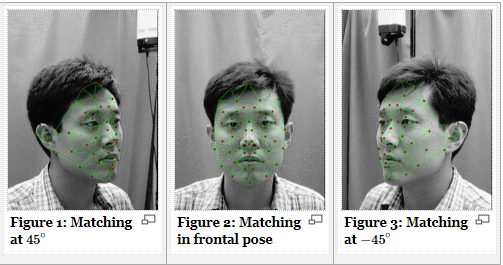
\includegraphics[scale=0.8]{resources/images/img/Face recognition/Elastic Bunch Graph Matching - Figures.png}
                    \caption{Aufbau eines Graphen im EBGM-Algorithmus [Quelle: \ref{scholarpedia:ebgm} / \ref{image:datapoints_of_a_EGBM_algoryhtm}]}
                    \label{fig:Datenpunkte_eines_EGBM-Algorithms}
                \end{figure}
            \end{center}
            Der Algorithmus selbst ist eine Version der \enquote{Dynamic Link Machine}, welche eine Modell der Objekt-Erkennung in unserem Gehirn ist [vgl. \ref{scholarpedia:ebgm}]. Eine ausführliche Beschreibung der Dynamic Link Machine ist in [\ref{subsec:dynamic_link_machine}] zu finden.\\
            Beim EBGM werden Graphen auf ein Bild gelegt und Markante Punkte durch sogenannte Jets gekennzeichnet [siehe Abbildung \ref{fig:Datenpunkte_eines_EGBM-Algorithms}]. Diese Punkte sind in allen Gesichtern mit einer kleinen Tolleranz gleich. Die Punkte aller verarbeiteten Gesichter werden in einem sogenannten Bunch zusammengefasst.

            \subsubsubsection{Jets}
            \label{subsubsubsec:jets}
                \begin{wrapfigure}[10]{r}{0.25\textwidth}
                    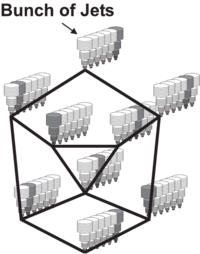
\includegraphics[width=0.25\textwidth]{resources/images/img/Face recognition/Elastic Bunch Graph Matching - Bunch of Jets.png}
                    \caption{Ansammlungen von Jets [Quelle \ref{image:Bunch_of_jets}]}
                    \label{fig:bunch_of_jets}
                \end{wrapfigure}
                Ein Jet bezeichnet eine geringe Menge an Grauwerten rund um ein definiertes Pixel. Diese beinhalten Informationen über die Gesichtstextur umliegend vom jeweiligen Punkt aus. Mit mehreren dieser Jets, lässt sich ein Graph bilden [siehe \ref{fig:bunch_of_jets}].

            \subsubsubsection{Graphs}
            \label{subsubsubsec:Graphs}
                Wie gerade in [\ref{subsubsubsec:jets}] schon erwähnt ist ein Graph eine Ansammlung von mehreren Jets. Hierbei werden die einzelnen Jets miteinander auf eine bestimmte Art und Weise mit einander verbunden.
\newpage
\section{Praktische Anwendung von Gesichtserkennung}
\label{sec:Praltische_Anwendung_Kuenslicher_Intelligenz}

    \subsection{Apples \enquote{Face-ID} und Androids \enquote{Trusted Face}}

    \subsection{Die Massenüberwachung in China}

    \subsection{Gesichtserkennung mit Developement-Boards}
\newpage
\section{Hinterfragen der Ethischen Korrektheit}
    In dieser Arbeit wurde neben dem Theoretischen Hintergrund [siehe \ref{sec:theorie}] auch auf die Praktische Anwendung in realen Systemen wie Smartphones [siehe \ref{subsec:FaceID_TrustedFace}] oder sogar in ganzen Ländern [siehe \ref{China:Massenueberwachung}] eingegangen. In dem folgendem Abschnitt wird nun die Ethische Korrektheit dieser Systeme untersucht. Hierbei wird sich vorallem auf die Seiten 312 & 313 der Quelle [\ref{book:religionsbuch_oberstufe}] bezogen.

    \subsection{Hinterfragen des Systems einer Künstlichen Intelligenz}
    \label{subsec:ethik_ki}
        Künstliche Intelligenz ist, wie man in dieser Facharbeit gesehen hat, ein sehr komplexes Themengebiet. Nicht unbedingt anders sieht es hier bei dem Hinterfragen der Ethischen Korrektheit von eben einer solchen KI.\\

        Betrachtet man zunächst die Nutzensethik so ist KI wohl mit eine der Theoretischen und Praktischen Systeme die hier den größten Zuspruch bekommen. Da sich die Nutzungsethik wirklich nur auf den Nutzen von etwas für den einzelnen oder die Gesellschaft bezieht kann man sich voll und ganz auf die positiven Seiten der Argumente konzentieren. Wie in [\ref{subsubsec:machnine_learning}] erfolgreich dargestellt wurde nützt uns KI schon in den alltäglichsten Dingen, wie z.B. eine neue Serie zum schauen finden die dem eigenen Interessengebiet entspricht. Auch ist Gesichtserkennung für die Sicherheit von Systemen sehr gut, aufgrund der Nutzung der biometrischen Daten eines Menschen, geignet wie es in [\ref{subsec:FaceID_TrustedFace} bzw. \ref{apple:face_id}] dargestellt wurde.\\

        Schaut man sich nun die weiteren Ethikformen an, fällt auf dass KI hier nicht unbedingt gut darsteht. Bei der Verantwortungsethik wird vorausgesetzt, dass auch Folgen des jeweiligen Handelns in die Entscheidung einfließen. Hierbei ist die Entscheidung ob es hier einen Ethischen Gewissenskonflikt gibt nicht einfach, da KI zwar lernfähig ist aber nur sinnvolle Entscheidungen für Situationen geben kann die sie trainiert hat. Somit stellt eine frisch programmierte KI, z.B. im Bereich des autonomen Fahrens, möglicherweise einen Ethischen Konflikt dar, da sie bestimmte Situationen einfach nicht beurteilen kann. Anders herum kann man aber argumentieren, dass eine langjährig trainierte KI diese Entscheidungen treffen kann. Hierbei ist allerdings zu beachten, dass es z.B. eine KI zum autonomen Fahren unmöglich alle möglichen Unfallszenarien durchlebt hat. Selbst wenn die KI über ein Netzwerk mit anderen Künstlichen Intelligenzen kommunizieren und lernen kann, so ist nicht zu 100\% sichergestellt, dass diese eine Entscheidung in einer kritischen Ausnahme Situation fällen kann. 
        
        Diese gleiche Situation sieht bei der Situationsethik allerdings anders aus. Hier wird nur auf die aktuelle Situation geschaut und nach dem bestmöglichen Ausgang für die KI gesucht. 

        \begin{wrapfigure}[10]{r}{0.25\textwidth}
            \centering
            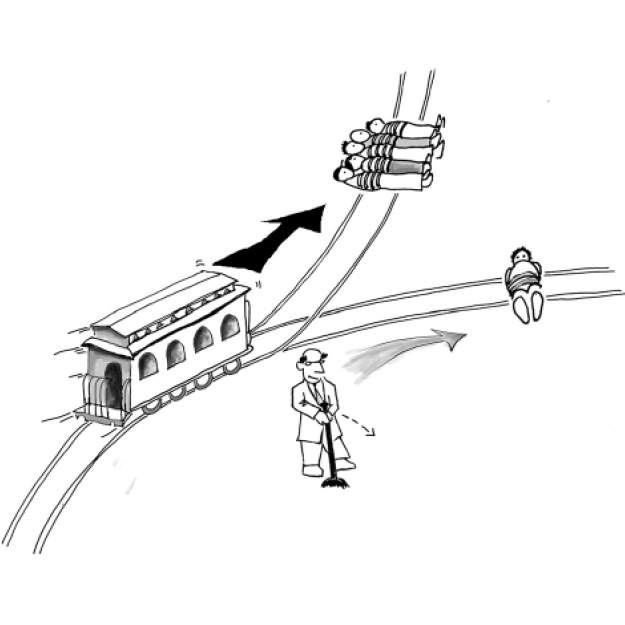
\includegraphics[width=0.25\textwidth]{resources/images/img/Gewissensfrage.jpg}
            \caption{\\[Quelle \ref{image:Gewissensfrage}]}
            \label{fig:Gewissensfrage}
        \end{wrapfigure}

        Als gutes Beispiel dient eine der Standard Gewissensfragen die normalerweise Menschen gestellt wird. Ein Zug fährt auf ein Gleis zu auf dem 4 Menschen liegen. Es gibt keine Möglichkeit ihn Aufzuhalten. Die einzige Möglichkeit diese Menschen noch zu retten ist die Weiche umzustellen. Allerdings liegt auf dem anderen Gleis auch eine Person. Die Frage: \enquote{Würdest du dir Weiche stellen?} [siehe Abbildung \ref{fig:Gewissensfrage}]\\

        Diese Frage ist für viele Menschen nicht einfach zu beantworten, da auf beiden Gleisen Menschen liegen. Eine KI würde hier relativ schnell ein Ergebnis fällen, je nachdem wie sie programmiert wurde. Höchstwahrscheinlich wird es die eine Entscheidung sein, welche den geringsten Schaden verursachen würde. Dabei würde die KI die Weiche stellen und 1 Menschenleben gegen 4 eintauschen. Auch wenn es für uns Menschen hart klingt entscheidet die KI nur Logisch.

    \subsection{Hinterfragen des Sozialpunktesystems in China}
        Im Gegensatz zu [\ref{subsec:ethik_ki}] muss bei der Ethik Hinterfragung des Sozialpunktesystems aus China keine KI die Fähigkeit zur ethischen Einschätzung haben, da es hier eher um die Frage ob es Ethisch Verantwortbar ist ein solches System für die Überwachung der Bevölkerung einzusetzen.\\
        
        Hierbei könnte die Gewissensethik durchaus als Basis der Diskussion dienen können. Allerdings würde in so einer Situation keine Antwort auf diese Frage finden, da die Gewissensethik von jedem Menschen einzeln abhängig ist.\\
        
        Vielmehr ergibt es sinn Hier auch mit der Nutzungsethik zu argumentieren. Zum einen gibt es einen großen Nutzen für Menschen mit einer hohen Punktzahl aber auch wiederum wenig Nutzen für Menschen mit einer niedrigen Punktzahl. Dieses System verpflichtet einen also fast schon dazu eine hohe Punktzahl zu besitzen, da man selbst sonst keinen Vorteil sondern sogar eher Nachteile daraus zieht.\\
        
        Andererseits ergibt sich daraus ein sehr großer Nutzen für die Gesellschaft, da der Großteil versuchen wird eine hohe Punktzahl zu erreichen. Da diese nicht durch unfaires Betrügen und Straftaten sondern dadurch gesteigert wird, dass man sich an Regeln hält, nett zu seinen Mitmenschen und sich für die Gesellschaft engagiert, hat dies eine drastische Reduzierung von Straftaten zufolge. Wobei dies auch mit der dauerhaften Überwachung in jedem Winkel zusammenhängt.
    
    \subsection{Fazit}
        Man kann Künstliche Intelligenz gut finden oder nicht. Was man aber nicht verneinen kann ist, dass KI uns in unserem Alltag schon so häufig begegnet wie es die meisten gar nicht stört sondern eher zufriedenstellt.\\
        
        Auf Basis der Nutzensethik kann man bei Künstlicher Intelligenz ganz klar von Ethischer Korrektheit reden. Das selbe gilt auch für die Situationsethik, da diese auf eine Logische neutrale Entscheidung angewiesen ist. Nur Bei der Gewissensethik kann KI, zu mindestens momentan, keine positives Ergebnis erreichen. Dies liegt ganz einfach daran, dass Computer kein Gewissen haben und wir momentan noch nicht in der Lage sind einem Computer ein Gewissen zu geben.
\newpage
\section{Literatur Verzeichnis}
\label{sec:literatur}

\subsection{Logic Theorist}
\label{bib:LogicTheorist}
	Letzter Zugriff: 12.02.2020\\
	URL: https://history-computer.com/ModernComputer/Software/LogicTheorist.html

	\subsubsection{Memorandum}
	\label{LogicTheorist:Memorandum}
		Letzter Zugriff: 18.02.2020 12:38\\
		URL: https://history-computer.com/Library/Logic\%20Theorist\%20memorandum.pdf
		
	\subsubsection{Wikipedia Artikel}
	\label{LogicTheorist:Wikipedia}
	Letzter Zugriff: 18.02.2020\\
	URL: https://en.wikipedia.org/wiki/Logic\_Theorist

\subsection{Allgemeine Quellen zum Thema KI}
\label{bib:AllgeimeineQuellen}
		\subsubsection{Wikipedia Artikel zum Thema Künstliche Intelligenz}
		\label{wiki:KuenstlicheIntelligenz}
		Letzter Zugriff: 19.02.2020 12:25\\
		URL: https://de.wikipedia.org/wiki/Künstliche\_Intelligenz

		\subsubsection{Gesichtserkennung}
		\label{wiki:face_recognition}
		Letzter Zugriff: 02.03.2020 17:19\\
		URL: https://de.wikipedia.org/wiki/Gesichtserkennung
	
\subsection{Aufbau und Funktionsweise Neuronaler Netze}		
\label{subsec:Aufbau_Funktion_Neuronaler_Netze}
		\subsubsection{JAAI - Aufbau von Neuronalen Netzen}
		\label{subsubsec:Aufbau_von_Neuronalen_Netzen}
		Letzter Zugriff: 22.02.22 15:04\\
		URL: https://jaai.de/kuenstliche-neuronale-netze-aufbau-funktion-291/

		\subsubsection{Wie lernen Neuronale Netze?}
		\label{subsubsec:Wie_lernen_neuronale_netze}
		Letzter Zugriff: 23.02.2020 17:49\\
		URL: https://jaai.de/machine-deep-learning-529/

\subsection{Bücher}
\label{books}

	\subsubsection{Buch: Digitale Gesichtserkennung}
	\label{book:DigitalGesichtserkennung}
		Untertitel: Theoretischer Überblick und praktische C++-Implementierung\\
		Autor: Andreas G. Ranftl\\
		Jahr: 2012\\
		Ort: Hamburg\\
		ISBN: 978-3-86341-432-0\\

	\subsubsection{Buch: Künstliche Intelligenz - Wann übernehmen die Maschinen?}
	\label{book:KI_WannUebernehmenDieMaschinen}
		Autor: Klaus Mainzer\\
		Jahr: 2016\\
		ISBN: 978-3-662-48452-4\\
		ISBN: 978-3-662-48453-1 (eBook)

	\subsubsection{Buch: Prinzipien der Mathematik}
	\label{book:prinzipa_of_mathmatics}
		Letzter Zugriff: 24.02.2020 12:14\\
		Autor: Bertrand Russel, Alfred North Whitehead\\
		URL: https://plato.stanford.edu/entries/principia-mathematica/

\subsection{Informationen über das menschliche Gehirn}
\label{subsec:Informationen_ueber_das_menschliche_Gehirn}
	\subsubsection{dasgehirn.info - Zellen: spezialisierte Arbeiter des Gehirns}
	\label{subsubsec:dasgehirn:Zellen-Arbeiter_Des_Gehrins}
	Letzter Zugriff: 22.02.2020 18:03\\
	URL: https://www.dasgehirn.info/grundlagen/kommunikation-der-zellen/zellen-spezialisierte-arbeiter-des-gehirns

\subsection{Viola Jones Algorithmus}
\label{algoryhtm:viola_jones}
	Letzter Zugriff: 02.03.2020 12:52\\
	URL: https://pdfs.semanticscholar.org/40b1/0e330a5511a6a45f42c8b86da222504c717f.pdf

\subsection{Facial Recognition}
\label{source:searchenterpriseai:facial_recognition}
	Letzter Zugriff: 02.03.2020 13:47\\
	URL: https://searchenterpriseai.techtarget.com/definition/facial-recognition

	\subsubsection{Elastic Bunch Graph Matching}
	\label{scholarpedia:ebgm}
	Letzter Zugriff: 02.03.2020 19:42\\
	URL: http://www.scholarpedia.org/article/Elastic\_Bunch\_Graph_Matching


\subsection{\enquote{Machine Learning} und \enquote{Deep Learning}}
\label{subsec:machine_learning_and_deep_learning}
	Letzter Zugriff: 01.03.2020 22:22\\
	URL: https://www.zendesk.com/blog/machine-learning-and-deep-learning/

\subsection{Netflix Research}
\label{Netlfix_Research}
	\subsubsection{Machine Learning - Learn hoe to entertain the World}
	\label{Netflix_Research:machine_learning_learn_how_to_entertain_the_world}
	Letzter Zugriff: 02.03.2020\\
	URL: https://research.netflix.com/research-area/machine-learning

\subsection{Bilder}
\label{subsec:Bilder_Anhang}
	\subsubsection{Beispiel eines Neuronalen Netzes}
	\label{subsubsec:Beispiel_eines_Neuronalen_Netzes}
	Download am: 22.02.2020 15:20\\
	URL: https://de.cleanpng.com/png-jxw2np/


% Bibliografie im .bib Format einfügen
\bibliography{bachelorarbeit}

\end{document}
